% week13_tue_boolean_binary.tex -- DSCT Tuesday, Nov 10 2026 (schedule change by Jeremy).
% Built from: Jeremy's plan 2026-11-10; week-14/student/tuesday-activity.md (truth-table check);
% lessons/12-boolean-algebra.md. Every number below was recomputed in Python
% (see check_numbers.py in this folder). Symbols are drawn in TikZ, no emoji fonts.
\documentclass[aspectratio=169,10pt]{beamer}
\usetheme{Madrid}
\usepackage{tikz}
\usepackage{amssymb}
\usetikzlibrary{circuits.logic.US,positioning,shapes.geometric}
\newcommand{\sO}{\tikz[baseline=-0.6ex]\draw[thick](0,0)circle(0.14);}
\newcommand{\sS}{\tikz[baseline=-0.6ex]\node[star,star points=5,star point ratio=2.2,draw,fill=yellow!70,inner sep=1pt]{};}
\newcommand{\sF}{\tikz[baseline=-0.6ex]{\draw[thick,fill=yellow!50](0,0)circle(0.15);\fill(-0.05,0.04)circle(0.015);\fill(0.05,0.04)circle(0.015);\draw(-0.07,-0.04)to[bend right=60](0.07,-0.04);}}
\newcommand{\sH}{\tikz[baseline=-0.6ex]{\draw[thick,fill=cyan!40](0,0)ellipse(0.16 and 0.09);\draw[thick,fill=cyan!40](0.14,0)--(0.27,0.1)--(0.27,-0.1)--cycle;\fill(-0.08,0.02)circle(0.015);}}
\newcommand{\bigsym}[1]{{\Large #1}}
\title{Counting, Carrying, and Circuits}
\subtitle{Week 13 Tuesday --- Boolean algebra, and how a computer adds and multiplies}
\author{COMSC 2043 \textbullet\ Discrete Structures and Critical Thinking}
\date{November 10, 2026}
\begin{document}

\frame{\titlepage
\note{75 minutes. Schedule change: Boolean algebra moved up to today; trees are out of this week; Thursday is Show \& Tell. Arc of the day: we already know how to carry in decimal. Strip the digits away and the same carrying works in any base. Binary is the base with two symbols. Then a Boolean circuit can do that carrying. Spine of evidence for the day: Sources, Rules/Assumptions, Work, Check, One-Sentence Summary.}}

\begin{frame}{Today's destination}
\begin{itemize}
\item Notice what \textbf{carrying} really is, using the decimal addition you already know.
\item See that any set of symbols can be a number system (circles, stars, faces, fish).
\item Add and multiply in \textbf{binary}, and see it is the same method as the one you learned.
\item Meet Boolean algebra and build a \textbf{half adder} and a \textbf{full adder} from it.
\end{itemize}
\note{Run of show: 0:00 warm-up and AI check (8). 0:08 decimal carrying (10). 0:18 octal and hex (10). 0:28 invented symbols (8). 0:36 binary add (8). 0:44 binary multiply (8). 0:52 Boolean algebra (8). 1:00 half and full adder (12). 1:12 exit ticket (3).}
\end{frame}

\begin{frame}{Warm-up: what happens at 9 + 1?}
Count on your fingers or on paper, out loud if you like:
\begin{center}\Large 7 + 1 \quad 8 + 1 \quad 9 + 1 \quad 99 + 1\end{center}
\begin{itemize}
\item What did you \emph{run out of} at 9 + 1?
\item Where did the extra digit come from?
\end{itemize}
\note{Let them say it: we ran out of digits. There is no single symbol bigger than 9, so we write a zero in the ones place and put a one in a new column. Do not give the word ``carry'' yet; let a student produce it.}
\end{frame}

\begin{frame}{Counting from 1 to 10 in decimal}
\begin{center}
\begin{tabular}{ccccccccccc}
0&1&2&3&4&5&6&7&8&9&\textbf{10}
\end{tabular}
\end{center}
\begin{itemize}
\item We have \textbf{ten} symbols: 0 through 9. Not 10 symbols plus ``10''.
\item At the end of the symbols, we \textbf{reset the ones place to 0} and \textbf{add 1 to the next place}.
\item The ``10'' is two digits: a 1 in the tens place and a 0 in the ones place.
\end{itemize}
\note{Hit the point: 10 is not a new symbol. It is a one and a zero, two digits. The first time we need a second column is exactly when the first column runs out. Odometer picture: the right wheel hits 9, rolls over to 0, and bumps the next wheel by one.}
\end{frame}

\begin{frame}{The same move at 99 + 1}
\begin{columns}
\column{0.45\textwidth}
\begin{center}
\begin{tabular}{r}
\texttt{\ \ 9\ 9}\\
\texttt{+\ \ \ 1}\\\hline
\texttt{1\ 0\ 0}
\end{tabular}
\end{center}
\column{0.55\textwidth}
\begin{enumerate}
\item $9+1$: ones place resets to 0, carry 1.
\item $9+1$ (the carry): tens place resets to 0, carry 1.
\item Nothing left to add to, so the carry becomes a new digit.
\end{enumerate}
\end{columns}
\vspace{4pt}
Place values: ones = $10^0$, tens = $10^1$, hundreds = $10^2$. \textbf{A new column appears every time the last one fills.}
\note{Walk it slowly. The carry ripples left. This ripple is the reason a circuit that adds is built from a chain of identical pieces; hold that thought for the full adder.}
\end{frame}

\begin{frame}{Check: use the carrying rule on bigger sums}
\begin{center}
\begin{tabular}{rr}
\texttt{\ 5\ 8}&\quad\texttt{\ 9\ 9\ 9}\\
\texttt{+\ 2\ 7}&\quad\texttt{+\ \ \ \ 1}\\\hline
\texttt{\ 8\ 5}&\quad\texttt{1\ 0\ 0\ 0}
\end{tabular}
\end{center}
Say aloud which columns carried, and what the carry is worth.
\note{58 + 27 = 85 (8+7 = 15: write 5, carry 1; 5+2+1 = 8). 999 + 1 = 1000 (three carries). Have two students narrate.}
\end{frame}

\begin{frame}{Octal: only eight symbols}
Digits \texttt{0 1 2 3 4 5 6 7}. There is no 8, no 9.
\begin{center}
\begin{tabular}{cccccccccc}
0&1&2&3&4&5&6&7&\textbf{10}&11
\end{tabular}
\end{center}
\begin{itemize}
\item At 7 + 1 we run out of symbols, so we write \texttt{10} (that number is \emph{eight}).
\item Same pattern at the next column: \texttt{77 + 1 = 100} (that number is \emph{sixty-four}).
\item Place values are powers of 8: $1,\ 8,\ 64,\ 512,\ \dots$
\end{itemize}
\note{Verified: 7+1 = 10 in octal (decimal 8). 77+1 = 100 in octal (decimal 64). Example sum in octal: 27 + 15 = 44 (7+5 = 12 decimal = 14 octal: write 4 carry 1; 2+1+1 = 4). Let the class check the last one.}
\end{frame}

\begin{frame}{Hexadecimal: sixteen symbols}
Digits \texttt{0 1 2 3 4 5 6 7 8 9 A B C D E F}. We borrow letters because we need six more symbols.
\begin{center}
\begin{tabular}{cccccccccccccccccc}
8&9&A&B&C&D&E&F&\textbf{10}&11
\end{tabular}
\end{center}
\begin{itemize}
\item \texttt{9 + 7 = 10}: sixteen, so a one and a zero. \texttt{A + 5 = F}.
\item \texttt{F + 1 = 10}. \texttt{FF + 1 = 100} (that number is two hundred fifty-six).
\item Place values: $1,\ 16,\ 256,\ 4096,\ \dots$
\end{itemize}
\note{Verified: hex 9+7 = 10 (decimal 16), hex A+5 = F, hex F+1 = 10, hex FF+1 = 100 (decimal 256). Example: 3B + 1C = 57 (B+C = 11+12 = 23 decimal = 17 hex: write 7, carry 1; 3+1+1 = 5). Why hex exists: one hex digit is exactly four binary digits, so it is shorthand for binary. Save that for the end of binary.}
\end{frame}

\begin{frame}{The pattern, in every base}
In base $b$ there are $b$ symbols, the biggest is $b-1$.
\begin{center}
\begin{tabular}{lcc}
 & \textbf{biggest digit $+1$} & \textbf{biggest two digits $+1$}\\\hline
base 10 & $9+1=10$ & $99+1=100$\\
base 8 & $7+1=10$ & $77+1=100$\\
base 16 & $F+1=10$ & $FF+1=100$
\end{tabular}
\end{center}
\textbf{``10'' always means one group of $b$ and none left over.} Only the name of the number changes.
\note{This is the generalization slide. If they have it, the invented-symbol slide is easy. Ask: what would this row look like for base 2? (1+1 = 10, 11+1 = 100.) Do not reveal yet, just ask and park it.}
\end{frame}

\begin{frame}{We do not need digits at all}
Four symbols: \quad \bigsym{\sO} \quad \bigsym{\sS} \quad \bigsym{\sF} \quad \bigsym{\sH}\quad (circle, star, face, fish)
\vspace{4pt}
Agree on an order: \bigsym{\sO} $<$ \bigsym{\sS} $<$ \bigsym{\sF} $<$ \bigsym{\sH}. That is a base-4 system.
\vspace{4pt}
\begin{itemize}
\item \bigsym{\sO} plays the role of 0, \bigsym{\sS} of 1, \bigsym{\sF} of 2, \bigsym{\sH} of 3.
\item After \bigsym{\sH}, we are out of symbols: next is \bigsym{\sS\,\sO} (``one group of four, none left'').
\end{itemize}
\note{This is the abstraction slide Jeremy asked for: a number system is a set of symbols plus an ordering plus the carry rule. The symbols are arbitrary. Ask the class to name the symbol that comes after fish-star-fish... wait for them to count.}
\end{frame}

\begin{frame}{Counting 0 to 8 with circles, stars, faces and fish}
\begin{center}
\begin{tabular}{rcl}
\textbf{decimal} & \textbf{base 4} & \textbf{symbols}\\\hline
0 & 0 & \bigsym{\sO} \\
1 & 1 & \bigsym{\sS} \\
2 & 2 & \bigsym{\sF} \\
3 & 3 & \bigsym{\sH} \\
4 & 10 & \bigsym{\sS\,\sO} \\
5 & 11 & \bigsym{\sS\,\sS} \\
6 & 12 & \bigsym{\sS\,\sF} \\
7 & 13 & \bigsym{\sS\,\sH} \\
8 & 20 & \bigsym{\sF\,\sO} \\
\end{tabular}
\end{center}
\note{Fill this in live if you want: cover the right column and let the class write it. Rows 0 through 8 here, 9 through 16 on the next slide.}
\end{frame}

\begin{frame}{Counting 9 to 16}
\begin{center}
\begin{tabular}{rcl}
\textbf{decimal} & \textbf{base 4} & \textbf{symbols}\\\hline
9 & 21 & \bigsym{\sF\,\sS} \\
10 & 22 & \bigsym{\sF\,\sF} \\
11 & 23 & \bigsym{\sF\,\sH} \\
12 & 30 & \bigsym{\sH\,\sO} \\
13 & 31 & \bigsym{\sH\,\sS} \\
14 & 32 & \bigsym{\sH\,\sF} \\
15 & 33 & \bigsym{\sH\,\sH} \\
16 & 100 & \bigsym{\sS\,\sO\,\sO} \\
\end{tabular}
\end{center}
Row 16 is the \bigsym{\sS\,\sO\,\sO} moment: the same thing as $99+1=100$.
\note{Decimal 16 is 100 in base 4 (one group of four fours). Same place-value story: ones, fours, sixteens.}
\end{frame}

\begin{frame}{Add in the invented system}
\begin{center}
\bigsym{\sH} $+$ \bigsym{\sS} $=$ \ ?\qquad\qquad \bigsym{\sH} $+$ \bigsym{\sH} $=$ \ ?
\end{center}
Translate to digits to check: \texttt{3 + 1 = 10} in base 4, which is \bigsym{\sS\,\sO}. \texttt{3 + 3 = 12} in base 4, which is \bigsym{\sS\,\sF}.
\begin{itemize}
\item Write the answer in the symbols, not the digits. The arithmetic does not care what the marks look like.
\end{itemize}
\note{Check: base-4 3+1 = 10 (decimal 4). Base-4 3+3 = 12 (decimal 6 = one four plus two). The lesson: the symbols were never the point. The rule about carrying was. This sets up: now use the smallest possible set of symbols.}
\end{frame}

\begin{frame}{Two symbols: binary}
Only \texttt{0} and \texttt{1}. Biggest digit is 1.
\begin{columns}
\column{0.3\textwidth}
\begin{tabular}{rl}
\textbf{n} & \textbf{binary}\\\hline
0 & \texttt{0} \\
1 & \texttt{1} \\
2 & \texttt{10} \\
3 & \texttt{11} \\
4 & \texttt{100} \\
5 & \texttt{101} \\
6 & \texttt{110} \\
7 & \texttt{111} \\
8 & \texttt{1000} \\
\end{tabular}
\column{0.3\textwidth}
\begin{tabular}{rl}
\textbf{n} & \textbf{binary}\\\hline
9 & \texttt{1001} \\
10 & \texttt{1010} \\
11 & \texttt{1011} \\
12 & \texttt{1100} \\
13 & \texttt{1101} \\
14 & \texttt{1110} \\
15 & \texttt{1111} \\
16 & \texttt{10000} \\
\end{tabular}
\column{0.38\textwidth}
Place values: $1,2,4,8,16,\dots$\\[6pt]
The first column fills at \texttt{1}. So \texttt{1 + 1 = 10} (that is two).
\end{columns}
\note{Pattern spotting: the ones column alternates 0 1 0 1; the twos column alternates in pairs; the fours in fours. Each column is half as fast as the one to its right. Verified table by Python. 8 = 1000, 16 = 10000.}
\end{frame}

\begin{frame}{Binary addition: the whole rule table}
\begin{center}
\begin{tabular}{c|c}
\textbf{sum} & \textbf{result}\\\hline
$0+0$ & \texttt{0}\\
$0+1$ & \texttt{1}\\
$1+0$ & \texttt{1}\\
$1+1$ & \texttt{10} \ (write 0, carry 1)
\end{tabular}
\end{center}
That is the entire addition table. With a carry in, the last case can reach $1+1+1=\texttt{11}$ (write 1, carry 1).
\note{Compare to decimal, where the table has 100 entries (10 by 10). Binary has four. Everything else is the carrying procedure they already know.}
\end{frame}

\begin{frame}[fragile]{Binary addition: worked examples}
\begin{columns}
\column{0.33\textwidth}
\begin{verbatim}
   11
 +  1
 -----
  100
\end{verbatim}
$3+1=4$
\column{0.33\textwidth}
\begin{verbatim}
  101
 +011
 -----
 1000
\end{verbatim}
$5+3=8$
\column{0.33\textwidth}
\begin{verbatim}
 1011
+0110
-----
10001
\end{verbatim}
$11+6=17$
\end{columns}
\vspace{4pt}
Carry from the right, one column at a time, exactly like decimal.
\note{Verified: 11+1 = 100 (3+1 = 4). 101+011 = 1000 (5+3 = 8). 1011+0110 = 10001 (11+6 = 17). Do the third one together, writing the carries above each column. Rightmost column 1+0 = 1; next 1+1 = 10 carry 1; next 0+1+1 = 10 carry 1; next 1+0+1 = 10 carry 1; the last carry becomes the new leftmost 1. Check by converting to decimal. Student tries: 0111 + 0101 (7+5 = 12 = 1100).}
\end{frame}

\begin{frame}{Check: your turn}
Add in binary, then convert both sides back to decimal to check.
\begin{center}
\texttt{0111 + 0101} \qquad\qquad \texttt{1111 + 0001}
\end{center}
One sentence: \textbf{where did each carry come from?}
\note{0111+0101 = 1100 (7+5 = 12). 1111+0001 = 10000 (15+1 = 16). The second one is the 99+1 moment again: every column carries. Ask them to say the phrase ``99 plus 1'' back.}
\end{frame}

\begin{frame}{Binary multiplication: the one-digit table}
\begin{center}
\begin{tabular}{c|c}
\textbf{product} & \textbf{result}\\\hline
$0\times0$ & \texttt{0}\\
$0\times1$ & \texttt{0}\\
$1\times0$ & \texttt{0}\\
$1\times1$ & \texttt{1}
\end{tabular}
\end{center}
A product of single bits is \textbf{1 only if both are 1}. Hold that thought: it is AND.
\note{Plant the connection now. Multiplication of bits = AND, and we will name it that in a few minutes.}
\end{frame}

\begin{frame}[fragile]{Binary long multiplication: same as the method you know}
\begin{columns}
\column{0.5\textwidth}
Decimal: $23\times 14=322$
\begin{verbatim}
    23
 x  14
 -----
    92   (23 x 4)
   230   (23 x 10)
 -----
   322
\end{verbatim}
\column{0.5\textwidth}
Binary: $5\times 3=15$
\begin{verbatim}
    101
 x   11
 ------
    101   (101 x 1)
   1010   (101 x 1, shifted)
 ------
   1111
\end{verbatim}
\end{columns}
\vspace{4pt}
Each partial product is either the top number or zeros, then shifted. Then \textbf{add}, using the rule table.
\note{Verified: 23 x 14 = 322; 101 x 11 = 1111 (5 x 3 = 15). Point out: in binary, each partial product is either a copy of the top number or all zeros, so there is no times table to memorize. Shifting left by one place is multiplying by two, the same way adding a zero on the right of 23 makes 230.}
\end{frame}

\begin{frame}[fragile]{More binary multiplication}
\begin{columns}
\column{0.5\textwidth}
\begin{verbatim}
    11
 x  10
 -----
    00
   110
 -----
   110
\end{verbatim}
$3\times2=6$
\column{0.5\textwidth}
\begin{verbatim}
    110
 x  101
 ------
    110
   0000
  11000
 ------
  11110
\end{verbatim}
$6\times5=30$
\end{columns}
\note{Verified: 11 x 10 = 110 (3 x 2 = 6). 110 x 101 = 11110 (6 x 5 = 30). Observe: multiplying by 10 (two) just shifts. Ask the class what multiplying by 100 does.}
\end{frame}

\begin{frame}{Where does a computer do this? Boolean algebra}
\textbf{Boolean algebra} has two values, true/false, which we write 1/0, and three basic operations:
\begin{center}
\begin{tabular}{c|c|c}
\textbf{AND} ($A\cdot B$) & \textbf{OR} ($A+B$) & \textbf{NOT} ($\overline{A}$)\\\hline
\begin{tabular}{cc|c}A&B&out\\\hline0&0&0\\0&1&0\\1&0&0\\1&1&1\end{tabular} &
\begin{tabular}{cc|c}A&B&out\\\hline0&0&0\\0&1&1\\1&0&1\\1&1&1\end{tabular} &
\begin{tabular}{c|c}A&out\\\hline0&1\\1&0\end{tabular}
\end{tabular}
\end{center}
\note{Compare AND with the one-bit multiplication table. They are identical. So single-bit multiplication is AND.}
\end{frame}

\begin{frame}{A trap: Boolean $1+1$ is not binary $1+1$}
\begin{columns}
\column{0.5\textwidth}
\textbf{In Boolean algebra} the plus sign means OR:
\[1+1=1\]
``true or true is true.''
\column{0.5\textwidth}
\textbf{In binary arithmetic} the plus sign means add:
\[1+1=10\]
one, one: write 0, carry 1.
\end{columns}
\vspace{6pt}
Same marks, different rules. \textbf{Always say which system you are in} (Sources, Rules/Assumptions).
\note{This is the critical-thinking beat of the day, and it is the usual Boolean-algebra stumble. The notation shares a plus sign. Ask: if I write 1 + 1 = 1, is that wrong? It depends on the Rules/Assumptions line. Link to the course habit: define terms before judging a claim.}
\end{frame}

\begin{frame}{A fourth gate: XOR (exclusive or)}
XOR is true when the inputs \textbf{differ}. Written $A\oplus B$.
\begin{center}
\begin{tabular}{cc|c|c}
A&B&\textbf{XOR}&\textbf{binary} $A+B$\\\hline
0&0&0&\texttt{00}\\
0&1&1&\texttt{01}\\
1&0&1&\texttt{01}\\
1&1&0&\texttt{10}
\end{tabular}
\end{center}
Look at the last two columns: the \textbf{right-hand digit of the sum is the XOR}, and the \textbf{left-hand digit (the carry) is the AND}.
\note{The key observation. The right digit of 0,1,1,0 is XOR's column. The left digit 0,0,0,1 is AND's column. So one bit of addition = one XOR gate for the sum bit and one AND gate for the carry bit. That is a half adder.}
\end{frame}

\begin{frame}{The half adder}
Adds two bits $A$ and $B$. Outputs: sum $S=A\oplus B$, carry $C=A\cdot B$.
\begin{columns}
\column{0.52\textwidth}
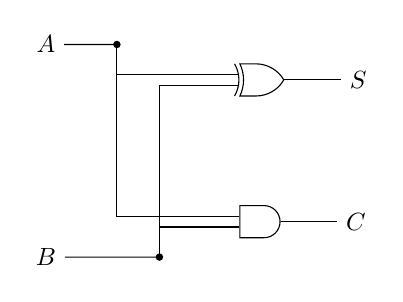
\begin{tikzpicture}[circuit logic US, every circuit symbol/.style={thick}, scale=0.9, transform shape]
\node[xor gate US, draw, logic gate inputs=nn] (x) at (3,1) {};
\node[and gate US, draw, logic gate inputs=nn] (a) at (3,-1) {};
\node (A) at (0,1.5) {$A$};
\node (B) at (0,-1.5) {$B$};
\draw (A.east) -- (1,1.5);
\draw (1,1.5) |- (x.input 1);
\draw (1,1.5) |- (a.input 1);
\draw (B.east) -- (1.6,-1.5);
\draw (1.6,-1.5) |- (a.input 2);
\draw (1.6,-1.5) |- (x.input 2);
\fill (1,1.5) circle (1.5pt);
\fill (1.6,-1.5) circle (1.5pt);
\draw (x.output) -- ++(0.8,0) node[right]{$S$};
\draw (a.output) -- ++(0.8,0) node[right]{$C$};
\end{tikzpicture}
\column{0.48\textwidth}
\begin{tabular}{cc|cc}
A&B&C&S\\\hline
0&0&0&0\\
0&1&0&1\\
1&0&0&1\\
1&1&1&0
\end{tabular}
\\[6pt]
Read $CS$ as a two-bit number: it equals $A+B$.
\end{columns}
\note{Every row of the table: A+B in binary is CS. 0+0 = 00, 0+1 = 01, 1+0 = 01, 1+1 = 10. The half adder cannot accept a carry coming in from the right, which is why it is called ``half''. Rubric habit: truth table is the evidence.}
\end{frame}

\begin{frame}[fragile]{The problem a half adder cannot solve}
Inside a long sum, every column after the first receives three bits: $A$, $B$, and the \textbf{carry-in} from the column to its right.
\begin{verbatim}
   1111      <- carries
    01101
  + 00111
  -------
   10100
\end{verbatim}
That is three inputs ($A$, $B$, $C_{in}$) and two outputs (sum, carry-out). We need a \textbf{full adder}.
\note{13 + 7 = 20. Column by column from the right: 1+1 = 10, carry 1; 0+1+1 = 10, carry 1; 1+1+1 = 11, write 1, carry 1; 1+0+1 = 10, carry 1; 0+0+1 = 1. Point at any middle column: three bits arrive.}
\end{frame}

\begin{frame}{The full adder}
Sum $S=A\oplus B\oplus C_{in}$. Carry-out $C_{out}=A\cdot B+C_{in}\cdot(A\oplus B)$.
\begin{columns}
\column{0.5\textwidth}
\begin{tabular}{ccc|cc}
A&B&$C_{in}$&$C_{out}$&S\\\hline
0&0&0&0&0\\
0&0&1&0&1\\
0&1&0&0&1\\
0&1&1&1&0\\
1&0&0&0&1\\
1&0&1&1&0\\
1&1&0&1&0\\
1&1&1&1&1
\end{tabular}
\column{0.5\textwidth}
Read $C_{out}S$ as a two-bit number: it equals $A+B+C_{in}$ in every row.\\[6pt]
Eight rows is every possible input. \textbf{Eight rows is a proof.}
\end{columns}
\note{Verified by brute force: all eight rows satisfy 2*Cout + S = A + B + Cin. This is the Week 14 theme pulled forward: a truth table over every assignment is a complete check, one passing assignment is not.}
\end{frame}

\begin{frame}{Full adder = two half adders and an OR}
\begin{center}
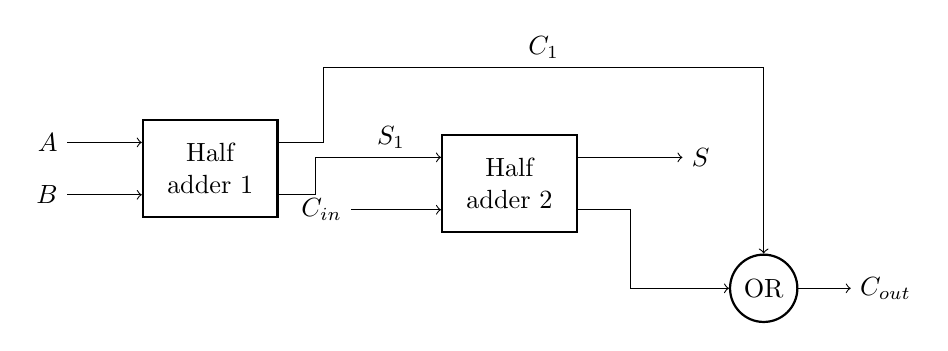
\begin{tikzpicture}[box/.style={draw,thick,minimum width=1.8cm,minimum height=1.3cm,align=center}, scale=0.95, transform shape]
\node[box] (h1) at (0,0) {Half\\adder 1};
\node[box] (h2) at (4,-0.2) {Half\\adder 2};
\node[draw,thick,circle,minimum size=0.9cm] (o) at (7.4,-1.6) {OR};
\draw[<-] ([yshift=0.35cm]h1.west) -- ++(-1,0) node[left]{$A$};
\draw[<-] ([yshift=-0.35cm]h1.west) -- ++(-1,0) node[left]{$B$};
\draw[->] ([yshift=-0.35cm]h1.east) -- ++(0.5,0) |- ([yshift=0.35cm]h2.west) node[pos=0.8,above]{$S_1$};
\draw[<-] ([yshift=-0.35cm]h2.west) -- ++(-1.2,0) node[left]{$C_{in}$};
\draw[->] ([yshift=0.35cm]h2.east) -- ++(1.4,0) node[right]{$S$};
\draw[->] ([yshift=-0.35cm]h2.east) -- ++(0.7,0) |- (o.west);
\draw[->] ([yshift=0.35cm]h1.east) -- ++(0.6,0) -- ++(0,1.0) -| (o.north) node[pos=0.25,above]{$C_1$};
\draw[->] (o.east) -- ++(0.7,0) node[right]{$C_{out}$};
\end{tikzpicture}
\end{center}
\textbf{Half adder 1} adds $A+B$. \textbf{Half adder 2} adds that sum plus $C_{in}$. Either one can make a carry, so OR combines them.
\note{If this diagram looks busy in the room, drop it and say it in words: first add A and B, then add the carry-in to that sum, and either step may produce a carry, so Cout = C1 OR C2. The two carries can never both be 1, which you can show with the truth table if time remains.}
\end{frame}

\begin{frame}{Chain them: a 4-bit ripple-carry adder}
\begin{center}
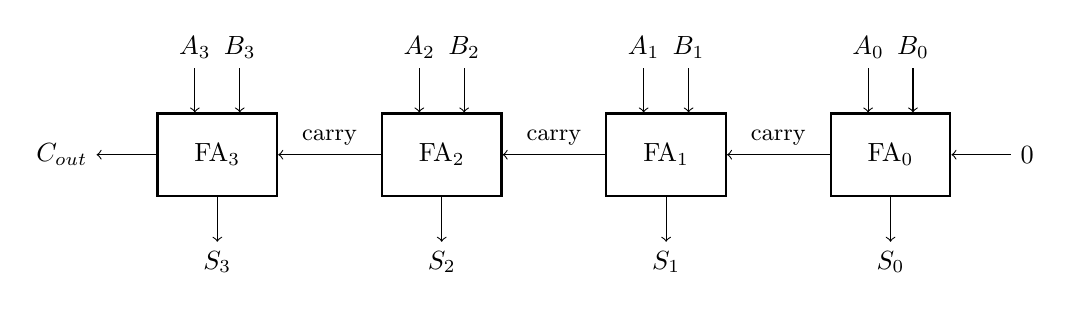
\begin{tikzpicture}[fa/.style={draw,thick,minimum width=1.6cm,minimum height=1.1cm}, scale=0.95, transform shape]
\foreach \i/\x in {0/9,1/6,2/3,3/0}{
  \node[fa] (f\i) at (\x,0) {FA$_\i$};
  \draw[<-] ([xshift=-0.3cm]f\i.north) -- ++(0,0.6) node[above]{$A_\i$};
  \draw[<-] ([xshift=0.3cm]f\i.north) -- ++(0,0.6) node[above]{$B_\i$};
  \draw[->] (f\i.south) -- ++(0,-0.6) node[below]{$S_\i$};
}
\draw[<-] (f0.east) -- ++(0.8,0) node[right]{$0$};
\foreach \i/\j in {0/1,1/2,2/3}{ \draw[->] (f\i.west) -- (f\j.east) node[midway,above]{\small carry}; }
\draw[->] (f3.west) -- ++(-0.8,0) node[left]{$C_{out}$};
\end{tikzpicture}
\end{center}
Each carry ripples left, one stage at a time: the same ripple as $99+1=100$.
\note{Example: 0111 + 0101. FA0: 1+1 = 10, write 0 carry 1. FA1: 1+0+1 = 10, write 0 carry 1. FA2: 1+1+1 = 11, write 1 carry 1. FA3: 0+0+1 = 1. Result 1100 = 12. Overflow: if the answer needs more bits than we built, the carry-out is lost. 1111 + 0001 on a 4-bit adder gives 0000 with Cout = 1. Ask: so what is 4-bit 15 + 1? It wraps. Real computers use wider adders but the same idea. Multiplication in hardware is shifting plus these adders, with AND gates making the partial products.}
\end{frame}

\begin{frame}{Putting multiplication in the circuit}
\begin{itemize}
\item Each partial product bit is an \textbf{AND} of one bit from each number.
\item Shifting is just wiring each row one place to the left.
\item The rows are added with \textbf{full adders}.
\end{itemize}
So a binary multiplier is AND gates plus the adders we just built.
\note{Closing the loop on the multiplication slides. Do not draw the full array multiplier unless asked; the point is that nothing new was added. Everything was AND, XOR, OR. The connection to traditional multiplication: same partial products, same shifts, same final add.}
\end{frame}

\begin{frame}{AI Fluency check}
An AI says:\ ``$A+B$ simplifies to $A$ because it worked for $A=1,\ B=1$.''
\begin{itemize}
\item Which system is the plus sign in: Boolean OR or binary addition?
\item Is one satisfying row a proof? What would be?
\end{itemize}
\textbf{Write one sentence}: what does a complete truth table prove that a single example cannot?
\note{Target: one passing row is a witness for ``there exists'' and says nothing about ``for all''. A full truth table over every input is a proof for a finite domain. And the plus sign is ambiguous until the system is named. This foreshadows Week 14's equivalence checks.}
\end{frame}

\begin{frame}{Exit ticket and Thursday}
\textbf{Exit ticket (one sentence each):}
\begin{enumerate}
\item In your own words: what does ``carry'' mean?
\item Which gate adds one bit, and which gate makes the carry?
\end{enumerate}
\vspace{6pt}
\textbf{Thursday:} Show \& Tell. \quad \textbf{Next Tuesday:} finite-state machines (coin machine, and more) with Mermaid diagrams.
\note{Answers: carry = when a place fills (reaches the base), reset it to 0 and add one to the next place. XOR gives the sum bit; AND gives the carry bit. Collect or ask for a show of fingers. Thursday is Show \& Tell, as arranged.}
\end{frame}

\end{document}
